\documentclass[11pt,a4paper]{article}
\usepackage[margin=2cm]{geometry}
\usepackage{graphicx,booktabs,hyperref,caption,multirow,array,float,amsmath}
\usepackage[font=small,labelfont=bf]{caption}
\usepackage{setspace}\onehalfspacing
\hypersetup{colorlinks=true,linkcolor=blue,urlcolor=blue}
\renewcommand{\figurename}{Fig.}
\renewcommand{\thefigure}{S\arabic{figure}}
\renewcommand{\thetable}{S\arabic{table}}
\usepackage{verbatim}

\title{\textbf{Supplementary Information}\\[0.3em]
\large Delta Dependency Prioritizes Paralog-Based Synthetic Lethality Candidates Across Solid Tumor Types}
\author{}
\date{}

\begin{document}

% --- Custom title block ---
\begin{center}
{\LARGE\bfseries Supplementary Information\par}
\vspace{0.5em}
{\large Delta Dependency Prioritizes Paralog-Based\\[0.2em] Synthetic Lethality Candidates Across Solid Tumor Types\par}
\vspace{1.2em}

{\large Qingqing Mo$^{1,2}$, Tao Zhu$^{1,2,\ast}$\par}
\vspace{0.6em}

{\small
\begin{tabular}{p{0.85\textwidth}}
$^{1}$ Department of Obstetrics and Gynecology, National Clinical Research Center for Obstetrics and Gynecology, Tongji Hospital, Tongji Medical College, Huazhong University of Science and Technology, Wuhan, China\\[0.3em]
$^{2}$ Key Laboratory of Cancer Invasion and Metastasis (Ministry of Education), Hubei Key Laboratory of Tumor Invasion and Metastasis, Tongji Hospital, Tongji Medical College, Huazhong University of Science and Technology, Wuhan, China
\end{tabular}\par}
\vspace{0.6em}

{\small $^{\ast}$ Correspondence: \texttt{zhutao@tjh.tjmu.edu.cn}\par}
\end{center}

\maketitle
\vspace{-2em}
\newpage
\tableofcontents
\newpage

\section{Supplementary Figures}

% S1
\begin{figure}[H]
\centering
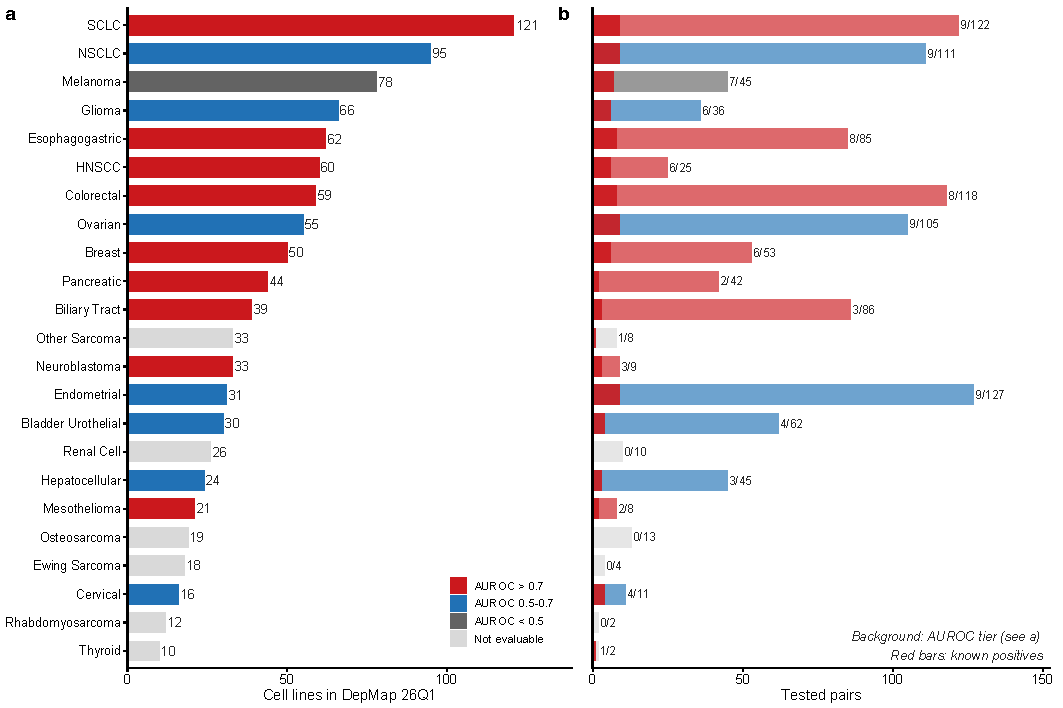
\includegraphics[width=\textwidth,height=0.45\textheight,keepaspectratio]{output/figures/FigS1_CellLine_Landscape.pdf}
\caption{\textbf{Cell line landscape and evaluation summary across 23 solid tumor types.} a, Cell line counts per cancer type, colored by DD AUROC tier (red: AUROC~$>$~0.7; blue: 0.5--0.7; gray: $<$~0.5; light gray: not evaluable). b, Tested paralog pairs per cancer type; red bars show known gold-standard positives. Numbers indicate known/total pairs.}
\end{figure}

% S2
\begin{figure}[H]
\centering
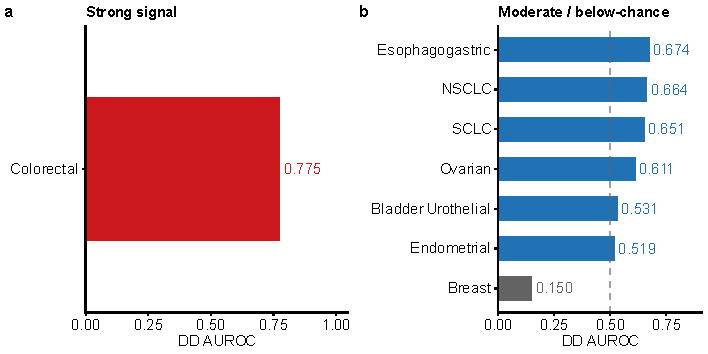
\includegraphics[width=\textwidth,height=0.45\textheight,keepaspectratio]{output/figures/FigS2_CrossCancer_AUROC.pdf}
\caption{\textbf{Cross-cancer DD AUROC.} DD AUROC for each of the 14 evaluable solid tumor types, grouped by signal strength. a, Strong signal (AUROC~$\ge$~0.7; 10 lineages including Biliary Tract 0.990, Esophagogastric 0.969, Pancreatic 0.949). b, Moderate signal (AUROC 0.5--0.7; Endometrial 0.690, Ovarian 0.651). c, Weak signal (AUROC~$<$~0.5; Melanoma 0.481, Cervical 0.476). Dashed line indicates random classifier (0.5). Bar labels show the number of tested paralog pairs per lineage. Cancer types with $<$2 known positive pairs were excluded from AUROC evaluation (see Table~S1 for the 9 non-evaluable types).}
\end{figure}

% S3
\begin{figure}[H]
\centering
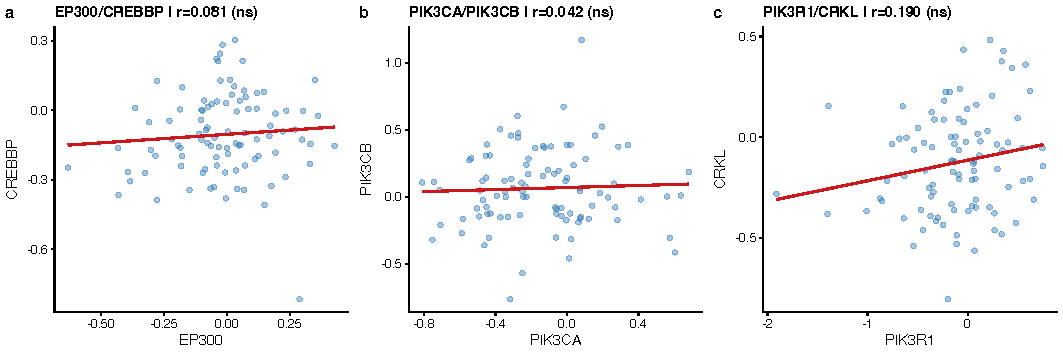
\includegraphics[width=\textwidth,height=0.45\textheight,keepaspectratio]{output/figures/FigS3_CPTAC_PerCohort.pdf}
\caption{\textbf{CPTAC per-cohort scatter plots (UCEC).} Representative scatter plot of EP300 vs.\ CREBBP protein abundance (log$_2$ normalized intensity) in the UCEC cohort ($n=83$). Each point represents one tumor sample. Line: linear regression fit with 95\% confidence band. Pearson $r$ and BH-corrected $q$-value shown. Similar scatter plots for other cohorts and paralog pairs are available upon request.}
\end{figure}

% S4
\begin{figure}[H]
\centering
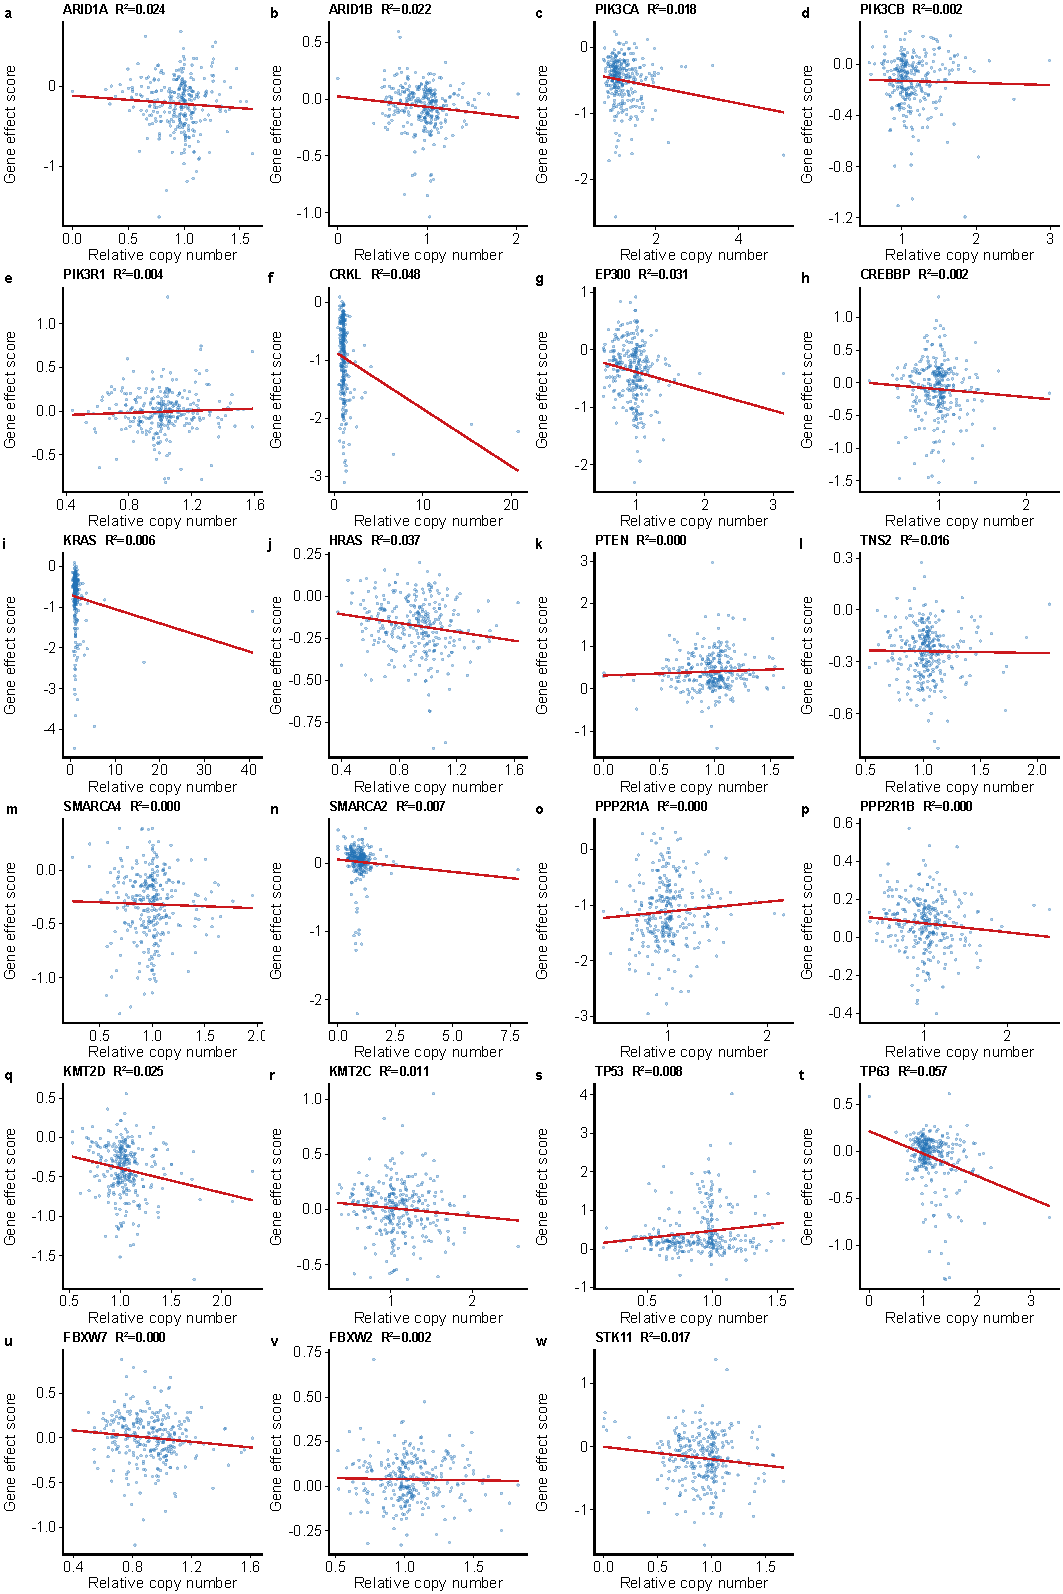
\includegraphics[width=\textwidth,height=0.7\textheight,keepaspectratio]{output/figures/FigS4_CNV_Independence.pdf}
\caption{\textbf{CNV independence analysis.} Scatter plots of relative copy number (x-axis) vs.\ Chronos gene-effect score (y-axis) for each of 23 paralog genes across 1,192 cell lines with both CNV and dependency data. Each panel shows one gene with the linear regression fit (red line) and $R^2$ value. All $R^2 < 0.10$, indicating that copy number variation explains $<$10\% of gene-effect variance. Multivariate regression controlling for driver mutation and TP53 co-mutation left DD estimates essentially unchanged after CNV adjustment (see main text).}
\end{figure}

% S5
\begin{figure}[H]
\centering
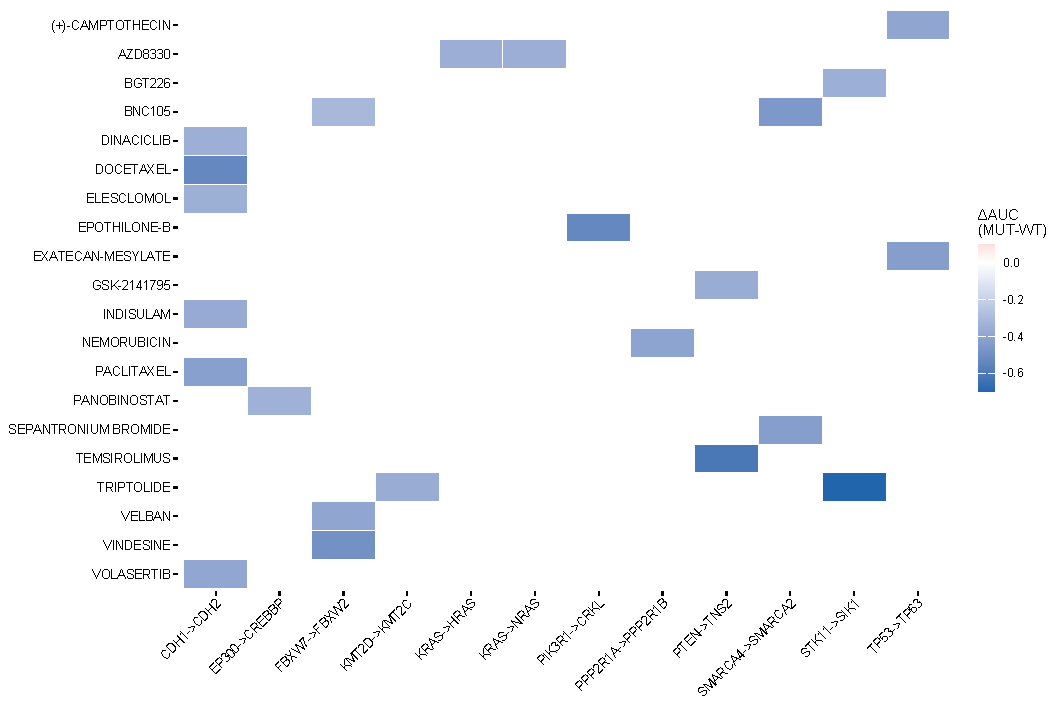
\includegraphics[width=\textwidth,height=0.55\textheight,keepaspectratio]{output/figures/FigS5_PRISM_Selectivity.pdf}
\caption{\textbf{PRISM drug selectivity heatmap.} Heatmap of drug sensitivity differential ($\Delta$AUC = mean AUC in driver-mutant minus mean AUC in wild-type cell lines) for the top compound--paralog pair associations from the PRISM Repurposing screen (1,482 compounds, 727 cell lines). Negative $\Delta$AUC indicates selective sensitivity in driver-mutant cells. Associations shown met discovery-stage criteria (BH $q<0.25$, $\Delta$AUC$<0$, enrichment$>0.1$). Known drug--target biology is recovered: MEK inhibitors with KRAS-mutant lines, mTOR/AKT inhibitors with PTEN-mutant lines, HDAC inhibitors with EP300-mutant lines.}
\end{figure}

% S6
\begin{figure}[H]
\centering
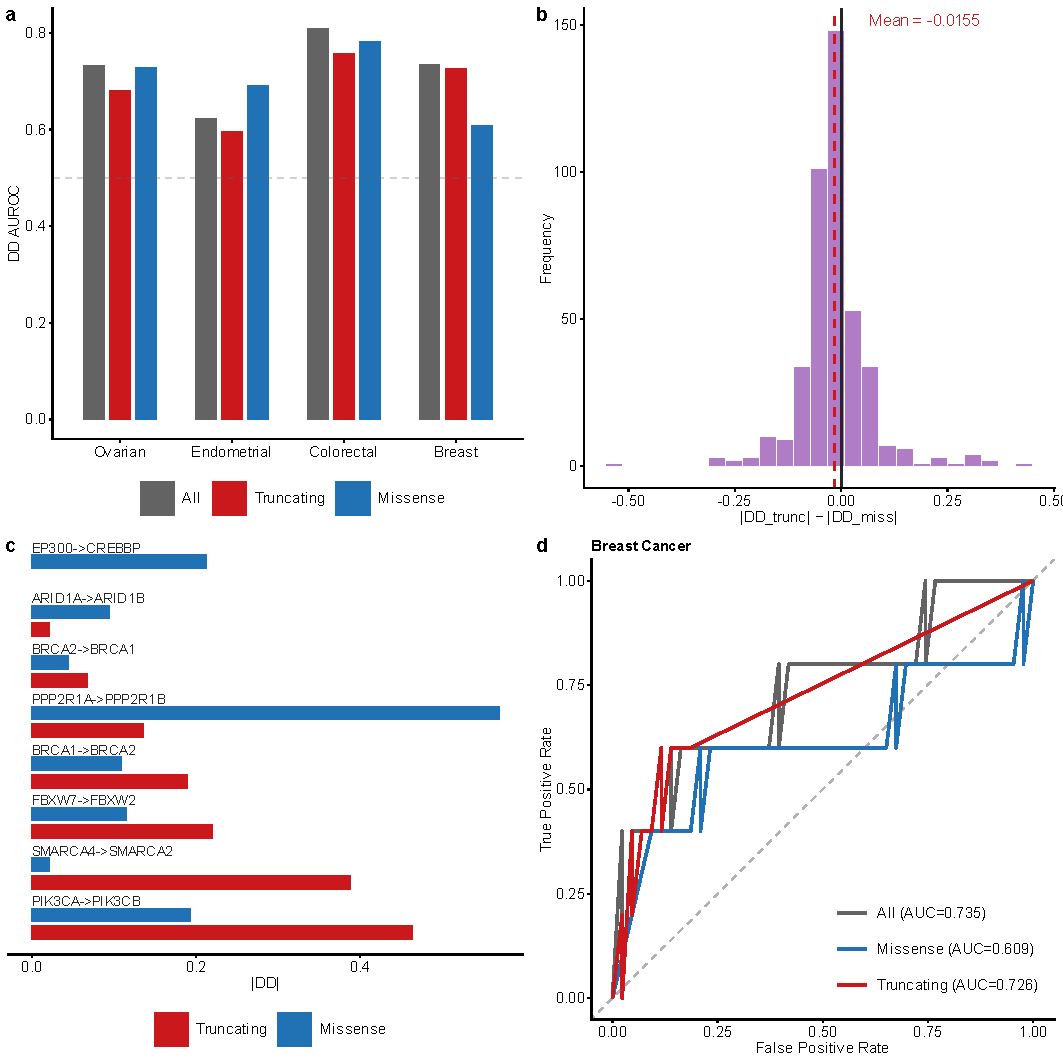
\includegraphics[width=\textwidth,keepaspectratio]{output/figures/FigS6_MutationType.pdf}
\caption{\textbf{Mutation-type stratification.} a, DD AUROC stratified by mutation type (truncating vs.\ missense) across cancer types. b, Distribution of $\Delta$DD (truncating minus missense) across all tested driver--paralog pairs; overall mean near zero ($-0.005$), indicating that truncating~$>$~missense is pair-specific rather than universal. c, $\Delta$DD for known gold-standard SL pairs showing that ARID1A$\rightarrow$ARID1B ($+0.368$ in Ovarian) and EP300$\rightarrow$CREBBP ($+0.314$ in Colorectal) drive the trend. d, ROC curves for Breast cancer comparing truncating-only (AUROC~$=$~0.726) vs.\ missense-only (0.391) and overall DD performance. Panel d is computed on the mutation-type analysis frame (48 Breast pairs); the resulting ``All'' AUC (0.735) therefore differs from the cross-cancer frame value (0.852; Fig.~1a), which uses a different pair universe.}
\end{figure}

% S7
\begin{figure}[H]
\centering
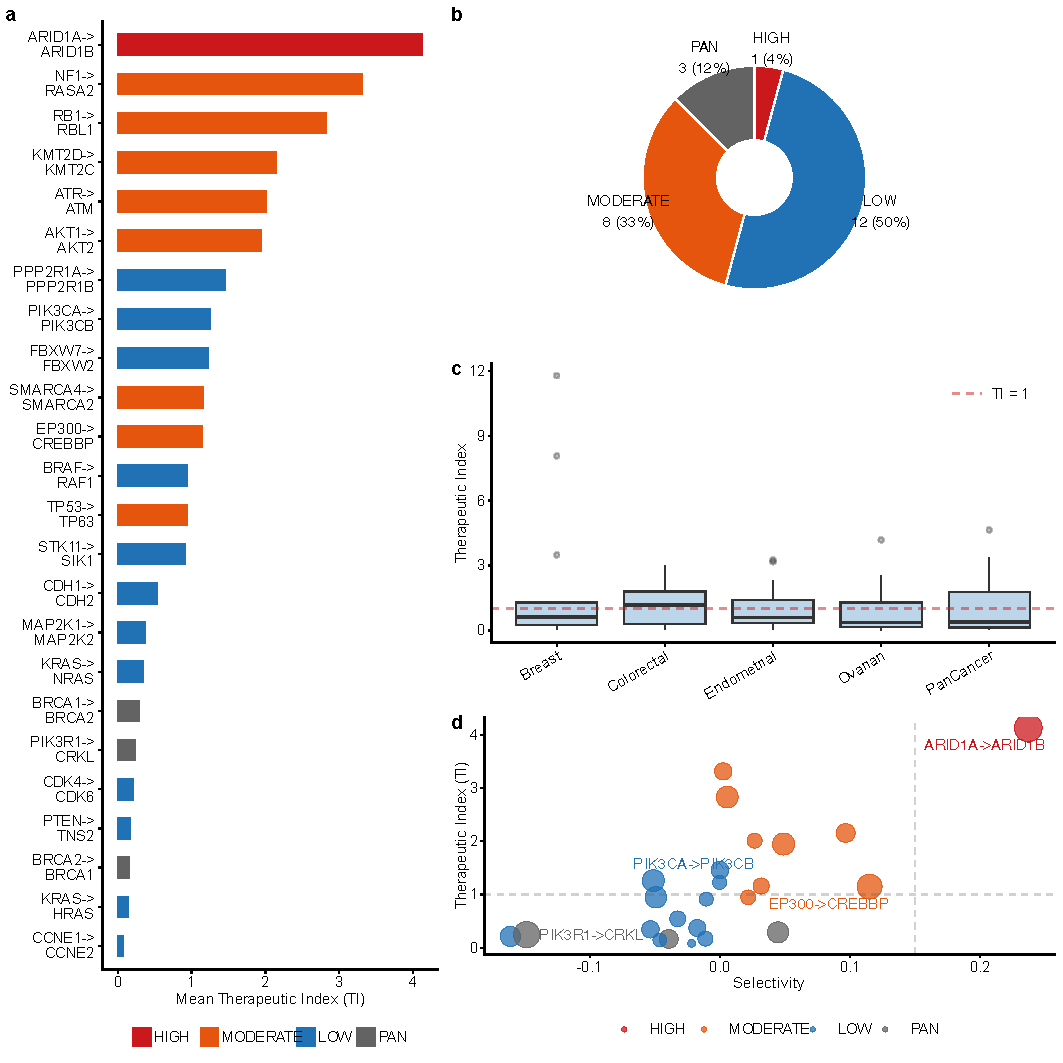
\includegraphics[width=\textwidth,keepaspectratio]{output/figures/FigS7_TherapeuticWindow.pdf}
\caption{\textbf{Therapeutic window analysis.} a, All 24 paralog pairs ranked by mean dependency window score (DWS) across 5 cancer contexts (Ovarian, Endometrial, Breast, Colorectal, PanCancer). ARID1A$\rightarrow$ARID1B ranks first (DWS~$=$~3.65). b, In vitro selectivity tier classification: HIGH\_SELECTIVITY (selectivity~$>$~0.15 and DWS~$>$~1.0), MODERATE, LOW\_SELECTIVITY, and PAN\_ESSENTIAL ($f_{\text{pan-essential}}>0.5$). c, DWS values broken down by individual cancer context showing cross-lineage consistency for top candidates. d, Selectivity vs.\ DWS scatter plot; ARID1A$\rightarrow$ARID1B is the only pair in the upper-right quadrant (high DWS and high selectivity).}
\end{figure}

% S8
\begin{figure}[H]
\centering
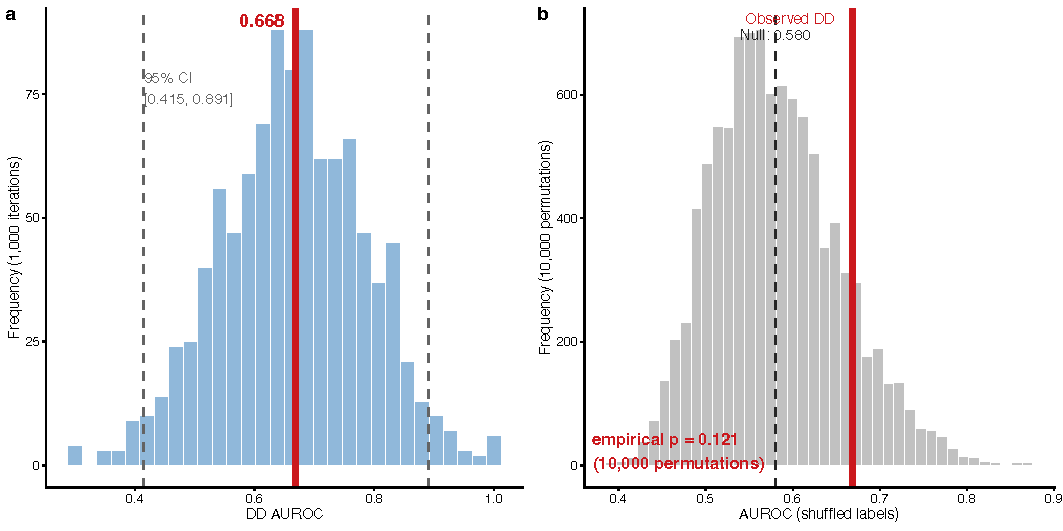
\includegraphics[width=0.7\textwidth,keepaspectratio]{output/figures/FigS8_Bootstrap_NegCtrl.pdf}
\caption{\textbf{Bootstrap and negative control (per-pair evaluation, 75 pairs, 6 known positives).} a, Bootstrap distribution (1,000 iterations; 95\% CI: 0.165--0.829). b, Null distribution from 10,000 label-shuffled permutations (empirical $p = 0.530$). The observed per-pair AUROC (0.493) does not exceed the null mean (0.501): with only 6 positive pairs the aggregated per-pair evaluation has no detectable signal, and the lineage-level evaluation (0.682, reported in the benchmark comparison) serves as the primary framework because it evaluates each driver$\times$paralog$\times$lineage combination separately rather than aggregating across lineages.}
\end{figure}

\begin{figure}[H]
\centering
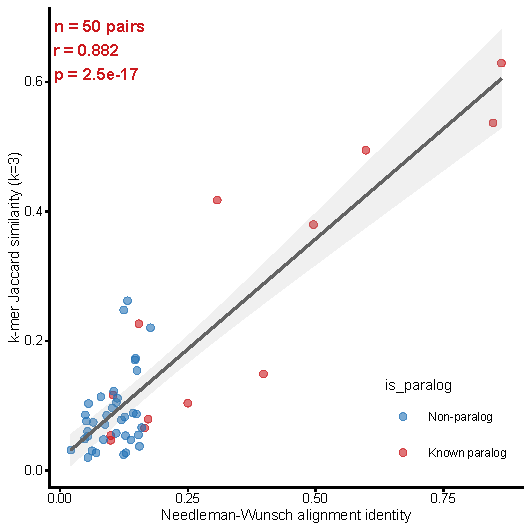
\includegraphics[width=0.45\textwidth,keepaspectratio]{output/figures/FigS9_kmer_validation.pdf}
\caption{\textbf{$k$-mer Jaccard vs.\ Needleman-Wunsch alignment identity validation.} Scatter plot of $k$-mer Jaccard similarity ($k=3$) vs.\ global alignment identity for 50 protein pairs (13 known paralogs, 37 non-paralog controls). Red: known paralog-SL pairs; Blue: non-paralog pairs. Gray line: linear regression with 95\% CI.}
\end{figure}

\begin{figure}[H]
\centering
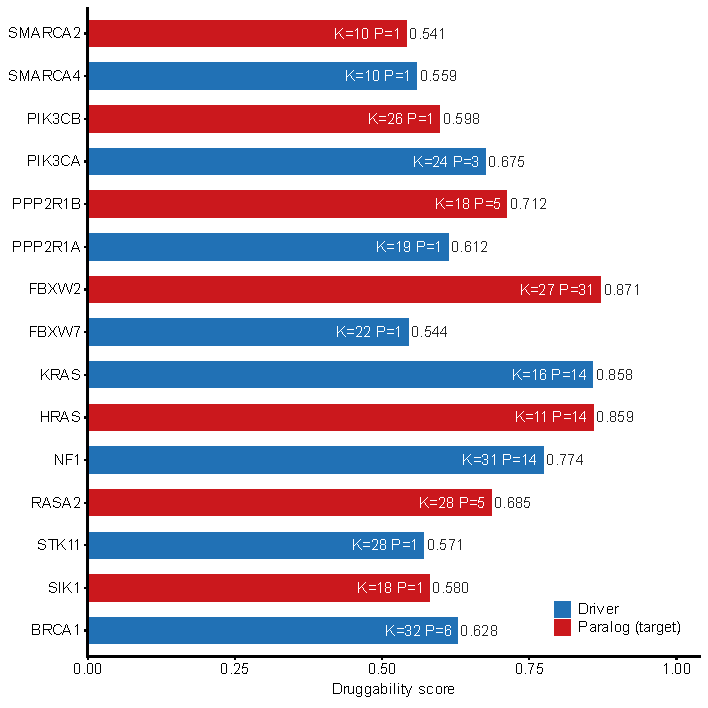
\includegraphics[width=0.65\textwidth,keepaspectratio]{output/figures/FigS10_Druggability.pdf}
\caption{\textbf{Structure-based druggability assessment.} Composite druggability score for 15 proteins (7 paralog targets in red, 8 driver genes in blue) based on ESMFold-predicted structures. Scores integrate structural confidence (pLDDT), hydrophobic content, lysine density (K, relevant for PROTAC conjugation), and predicted pocket count (P). Structures were limited to 400 residues per protein; ARID1A/ARID1B structures were not available from AlphaFold DB and are assessed by sequence-level features only (main text Table~2). FBXW2 (0.871) and KRAS/HRAS (0.858--0.859) show the highest scores due to well-folded compact domains.}
\end{figure}

\clearpage
\section{Supplementary Tables}

\subsection{Table S1: Cell line and evaluation summary across 23 solid tumor types}
\begin{table}[H]
\centering
\footnotesize
\setlength{\tabcolsep}{4.5pt}
\begin{tabular}{llrrrr}
\toprule
\textbf{Label} & \textbf{Full name} & \textbf{Cell Lines} & \textbf{Pairs} & \textbf{Known+} & \textbf{DD AUROC} \\
\midrule
Biliary Tract & Biliary tract cancer & 39 & 50 & 2 & 0.990 \\
Esophagogastric & \shortstack[l]{Esophagogastric adenocarcinoma /\\esophageal SCC} & 62 & 69 & 4 & 0.969 \\
Pancreatic & Pancreatic adenocarcinoma & 44 & 41 & 2 & 0.949 \\
Glioma & Diffuse glioma & 66 & 28 & 2 & 0.885 \\
Bladder Urothelial & Bladder urothelial carcinoma & 30 & 20 & 3 & 0.882 \\
Breast & Invasive breast carcinoma & 50 & 48 & 4 & 0.852 \\
HNSCC & Head and neck squamous cell carcinoma & 60 & 18 & 2 & 0.812 \\
SCLC & Small cell lung cancer & 121 & 107 & 6 & 0.779 \\
NSCLC & Non-small cell lung cancer & 95 & 104 & 6 & 0.738 \\
Colorectal & Colorectal adenocarcinoma & 59 & 76 & 8 & 0.726 \\
\midrule
Endometrial & Endometrial carcinoma & 31 & 77 & 6 & 0.690 \\
Ovarian & Ovarian epithelial carcinoma & 55 & 65 & 8 & 0.651 \\
Melanoma & Melanoma & 78 & 31 & 4 & 0.481 \\
Cervical & Cervical carcinoma & 16 & 10 & 3 & 0.476 \\
\midrule
Mesothelioma & Pleural mesothelioma & 21 & 5 & 1 & --- \\
Hepatocellular & Hepatocellular carcinoma & 24 & 7 & 1 & --- \\
Renal Cell & Renal cell carcinoma & 26 & 9 & 0 & --- \\
Neuroblastoma & Neuroblastoma & 33 & 6 & 1 & --- \\
Osteosarcoma & Osteosarcoma & 19 & 12 & 0 & --- \\
Ewing Sarcoma & Ewing sarcoma & 18 & 2 & 0 & --- \\
Rhabdomyosarcoma & Rhabdomyosarcoma & 12 & 2 & 0 & --- \\
Other Sarcoma & Other soft-tissue sarcoma & 33 & 6 & 1 & --- \\
Thyroid & Thyroid carcinoma & 10 & 2 & 1 & --- \\
\bottomrule
\end{tabular}
\caption{Cell line counts and DD AUROC across all 23 analyzed solid tumor types. Top: AUROC~$>$~0.7 (10 types). Middle: AUROC~$\le$~0.7 (4 types). Bottom: insufficient known positives for AUROC (9 types). Known+: number of gold-standard positive pairs evaluable in each lineage. ``---'': AUROC not computable ($<$2 known positives). Full name: standardized cancer-type name corresponding to each short label; SCC, squamous cell carcinoma.}
\end{table}

\subsection{Table S2: Complete paralog-SL pair analysis results}
The full analysis results are provided as a tab-separated file: \texttt{TableS2\_FullResults.tsv} (116 rows $\times$ 13 columns, representing all driver$\times$paralog$\times$cancer-type combinations passing the minimum sample-size filter).

\textbf{Data dictionary:}
\begin{itemize}\setlength\itemsep{0pt}
\item \texttt{driver\_gene}: Driver gene with damaging mutation.
\item \texttt{paralog\_gene}: Candidate paralog tested for conditional dependency.
\item \texttt{cancer\_type}: Solid tumor lineage (DepMap OncotreePrimaryDisease).
\item \texttt{pcs}: Paralog Compensation Score (DD $\times$ necessity).
\item \texttt{delta\_expression}: $\Delta$Expression between MUT and WT groups.
\item \texttt{necessity}: Mean gene-effect score of the paralog (more negative = more essential).
\item \texttt{dependency\_dd}: Delta Dependency (signed; positive = greater dependency in MUT).
\item \texttt{composite\_score}: Weighted composite of PCS, DD, and $\Delta$Expression.
\item \texttt{novelty}: ``Known'' if in gold-standard set (Table~S3), else ``Novel''.
\item \texttt{q\_value}: Benjamini-Hochberg adjusted $p$-value within each driver gene.
\item \texttt{mutation\_frequency}: Fraction of cell lines with driver mutation in this lineage.
\item \texttt{n\_mut}, \texttt{n\_wt}: Number of mutant and wild-type cell lines.
\item \texttt{is\_known\_paralog\_sl}: Boolean; TRUE if pair is in gold-standard set.
\end{itemize}
\stepcounter{table} % Table S2 has no \begin{table}, manually increment counter

\subsection{Table S3: Gold-standard paralog-SL pairs with evidence provenance and tier assignment}
\begin{table}[H]
\centering
\footnotesize
\resizebox{\textwidth}{!}{%
\begin{tabular}{llllllc}
\toprule
\textbf{Tier} & \textbf{Driver} & \textbf{Paralog} & \textbf{Type} & \textbf{Evidence} & \textbf{Key Ref} & \textbf{Indep.} \\
\midrule
A & SMARCA4 & SMARCA2 & Seq.\ paralog & CRISPR screen & Hoffman 2014 & Yes \\
A & ARID1A  & ARID1B  & Seq.\ paralog & CRISPR + drug & Helming 2014 & Yes \\
\midrule
A$^*$ & EP300 & CREBBP & Seq.\ paralog & Reciprocal SL (CREBBP$\rightarrow$EP300) & Ogiwara 2016; Nie 2021 & Yes \\
\midrule
comparator & BRCA1 & BRCA2 & Func.\ analog & Genetic screen & Bryant 2005 & Yes \\
comparator & STK11 & SIK1  & Partial hom.  & LKB1--SIK axis (mouse genetics) & Hollstein 2019 & Yes \\
\midrule
B & AKT1    & AKT2    & Seq.\ paralog & Digenic KO (comb.\ CRISPR) & Najm 2018 & Yes \\
B & CCNE1   & CCNE2   & Seq.\ paralog & Mouse double-KO redundancy & Geng 2003 & Yes \\
B & PIK3CA  & PIK3CB  & Seq.\ paralog & Redundancy/pharmacologic & Wee 2008 (PTEN$\rightarrow$PIK3CB only) & Yes \\
B & CDK4    & CDK6    & Seq.\ paralog & Digenic KO (pgPEN) + drug & Parrish 2021 & Yes \\
B & MAP2K1  & MAP2K2  & Seq.\ paralog & Digenic KO (pgPEN) + drug & Parrish 2021 & Yes \\
\midrule
C & FBXW7   & FBXW2   & Seq.\ paralog & DepMap analysis & DepMap & No \\
C & PPP2R1A & PPP2R1B & Seq.\ paralog & DepMap analysis & DepMap & No \\
\bottomrule
\end{tabular}%
}
\caption{Twelve curated pairs with evidence provenance and tier assignment. Tier A (2 pairs): directional external experimental evidence matching the direction scored here; used for directional claims. A$^*$ (1 pair): synthetic lethality experimentally established in the reciprocal direction only (CREBBP$\rightarrow$EP300); the direction scored here (EP300$\rightarrow$CREBBP) is supported by paralog redundancy alone, so the pair is excluded from directional Tier A claims and relabelled non-positive in the direction-strict sensitivity analysis. Comparator (2 pairs): mechanistic reference pairs (functional analog or pathway axis), reported separately. Tier B (5 pairs): paralog-redundancy, digenic-knockout, or pharmacologic evidence only, not directional genotype-conditional. Tier C (2 pairs): DepMap-derived, excluded from directional claims to avoid circularity. Type: Seq.\ paralog (shared gene family, conserved domains), Func.\ analog (shared pathway role, no sequence homology), Partial hom.\ (same superfamily, divergent). Indep.: whether evidence is independent of DepMap CRISPR data. ``No'' indicates pairs whose SL status was originally identified from DepMap-derived analyses, creating potential circularity.}
\end{table}

\subsection{Table S4: Pan-cancer summary statistics}
\begin{table}[H]
\centering
\footnotesize
\begin{tabular}{lrrr}
\toprule
\textbf{Cancer Type} & \textbf{Cell Lines} & \textbf{Pairs} & \textbf{DD AUROC} \\
\midrule
Biliary Tract        & 39 & 50 & 0.990 \\
Esophagogastric      & 62 & 69 & 0.969 \\
Pancreatic           & 44 & 41 & 0.949 \\
Glioma               & 66 & 28 & 0.885 \\
Bladder Urothelial   & 30 & 20 & 0.882 \\
Breast               & 50 & 48 & 0.852 \\
HNSCC                & 60 & 18 & 0.812 \\
SCLC                 & 121 & 107 & 0.779 \\
NSCLC                & 95 & 104 & 0.738 \\
Colorectal           & 59 & 76 & 0.726 \\
\midrule
Endometrial          & 31 & 77 & 0.690 \\
Ovarian              & 55 & 65 & 0.651 \\
Melanoma             & 78 & 31 & 0.481 \\
Cervical             & 16 & 10 & 0.476 \\
\bottomrule
\end{tabular}
\caption{DD AUROC across all 14 evaluable solid tumor types (sorted by AUROC). Horizontal line separates AUROC~$>$~0.7 (top, 10 lineages) from AUROC~$\le$~0.7 (bottom). Full lineage names are given in Table~S1.}
\end{table}

\subsection{Table S5: 40-gene driver panel}
\begin{table}[H]
\centering
\footnotesize
\begin{tabular}{llll}
\toprule
\textbf{Gene} & \textbf{Cancer Types} & \textbf{Source} & \textbf{Category} \\
\midrule
TP53 & Pan-cancer & TCGA+COSMIC & TSG \\
KRAS & Lung, CRC, Pancreatic & TCGA+COSMIC & Oncogene \\
PIK3CA & Breast, Endometrial, Cervical & TCGA+COSMIC & Oncogene \\
PTEN & Endometrial, Ovarian, Breast & TCGA+COSMIC & TSG \\
ARID1A & Endometrial, Ovarian, CRC & TCGA+COSMIC & TSG \\
BRCA1 & Ovarian, Breast & TCGA+COSMIC & TSG \\
BRCA2 & Ovarian, Breast & TCGA+COSMIC & TSG \\
BRAF & Melanoma, CRC, Thyroid & TCGA+COSMIC & Oncogene \\
NF1 & Glioma, Breast, Lung & TCGA+COSMIC & TSG \\
RB1 & SCLC, Breast, Bladder & TCGA+COSMIC & TSG \\
\bottomrule
\end{tabular}
\caption{First 10 of 40 driver genes (complete list in TableS5\_DriverGenes.tsv).
Selection criteria: recurrently mutated in $\ge$1 TCGA pan-cancer study or COSMIC Cancer Gene Census,
with $\ge$3 mutant cell lines in at least one DepMap lineage.}
\end{table}

\subsection{Table S6: All 24 paralog pairs ranked by preclinical prioritization score}
\begin{table}[H]
\centering
\footnotesize
\begin{tabular}{llrrrll}
\toprule
\textbf{Driver} & \textbf{Paralog} & \textbf{$|$DD$|$} & \textbf{DWS} & \textbf{Select.} & \textbf{Class} & \textbf{Type} \\
\midrule
ARID1A & ARID1B & 0.250 & 3.647 & 0.228 & HS & Seq \\
NF1 & RASA2 & 0.062 & 3.260 & 0.002 & MOD & Seq \\
KMT2D & KMT2C & 0.112 & 2.558 & 0.131 & MOD & Seq \\
ATR & ATM & 0.049 & 2.182 & 0.031 & MOD & Seq \\
RB1 & RBL1 & 0.112 & 2.059 & 0.003 & MOD & Seq \\
AKT1 & AKT2 & 0.119 & 1.657 & 0.036 & MOD & Seq \\
PPP2R1A & PPP2R1B & 0.068 & 1.454 & 0.000 & LS & Seq \\
SMARCA4 & SMARCA2 & 0.057 & 1.268 & 0.039 & MOD & Seq \\
PIK3CA & PIK3CB & 0.137 & 1.245 & $-$0.052 & LS & Seq \\
EP300 & CREBBP & 0.187 & 1.185 & 0.120 & MOD & Seq \\
FBXW7 & FBXW2 & 0.030 & 1.032 & 0.000 & LS & Seq \\
STK11 & SIK1 & 0.037 & 1.018 & $-$0.010 & LS & Part \\
BRAF & RAF1 & 0.105 & 0.824 & $-$0.038 & LS & Seq \\
CDH1 & CDH2 & 0.057 & 0.722 & $-$0.030 & LS & Seq \\
TP53 & TP63 & 0.031 & 0.690 & 0.036 & MOD & Seq \\
MAP2K1 & MAP2K2 & 0.067 & 0.401 & $-$0.017 & LS & Seq \\
KRAS & NRAS & 0.071 & 0.358 & $-$0.055 & LS & Seq \\
BRCA1 & BRCA2 & 0.125 & 0.290 & 0.046 & PE & Func \\
BRCA2 & BRCA1 & 0.094 & 0.177 & $-$0.039 & PE & Func \\
PTEN & TNS2 & 0.041 & 0.172 & $-$0.012 & LS & Seq \\
CDK4 & CDK6 & 0.079 & 0.157 & $-$0.121 & LS & Seq \\
KRAS & HRAS & 0.028 & 0.139 & $-$0.045 & LS & Seq \\
PIK3R1 & CRKL & 0.100 & 0.111 & $-$0.112 & PE & Seq \\
CCNE1 & CCNE2 & 0.004 & 0.060 & $-$0.022 & LS & Seq \\
\bottomrule
\end{tabular}
\caption{All 24 analyzed paralog pairs ranked by mean dependency window score (DWS). $|$DD$|$: mean absolute Delta Dependency across cancer contexts. Select.: mean selectivity (fraction mutant-essential minus fraction wild-type-essential). Class: HS=HIGH\_SELECTIVITY, MOD=MODERATE, LS=LOW\_SELECTIVITY, PE=PAN\_ESSENTIAL. Type: Seq=sequence paralog, Part=partial homology, Func=functional analog.}
\end{table}


\subsection{Table S7: Gene-class-specific driver-mutation rules and variant classification}
\begin{table}[H]
\centering
\footnotesize
\begin{tabular}{lllrrr}
\toprule
\textbf{Gene} & \textbf{Class} & \textbf{Rule} & \textbf{Old} & \textbf{New} & \textbf{\% ret.} \\
\midrule
ALK & ONC & Hotspot & 118 & 12 & 10.2 \\
APC & TSG & LikelyLoF & 217 & 108 & 49.8 \\
ARID1A & TSG & LikelyLoF & 240 & 173 & 72.1 \\
ATM & TSG & LikelyLoF & 165 & 59 & 35.8 \\
ATR & TSG & LikelyLoF & 125 & 37 & 29.6 \\
BRAF & ONC & Hotspot & 212 & 162 & 76.4 \\
BRCA1 & TSG & LikelyLoF & 101 & 34 & 33.7 \\
BRCA2 & TSG & LikelyLoF & 159 & 68 & 42.8 \\
CCNE1 & ONC & Hotspot & 22 & 0 & 0.0 \\
CDH1 & TSG & LikelyLoF & 87 & 34 & 39.1 \\
CDK4 & ONC & Hotspot & 27 & 8 & 29.6 \\
CTNNB1 & ONC & Hotspot & 85 & 45 & 52.9 \\
EGFR & ONC & Hotspot & 110 & 19 & 17.3 \\
EP300 & TSG & LikelyLoF & 206 & 107 & 51.9 \\
ERBB2 & ONC & Hotspot & 70 & 20 & 28.6 \\
FBXW7 & TSG & LikelyLoF & 116 & 81 & 69.8 \\
GATA3 & TSG & LikelyLoF & 52 & 16 & 30.8 \\
KEAP1 & TSG & LikelyLoF & 99 & 31 & 31.3 \\
KMT2D & TSG & LikelyLoF & 356 & 185 & 52.0 \\
KRAS & ONC & Hotspot & 254 & 233 & 91.7 \\
MAP2K1 & ONC & Hotspot & 36 & 14 & 38.9 \\
MAP3K1 & TSG & LikelyLoF & 74 & 14 & 18.9 \\
MAPK1 & ONC & Hotspot & 13 & 0 & 0.0 \\
MET & ONC & Hotspot & 66 & 1 & 1.5 \\
NF1 & TSG & LikelyLoF & 215 & 122 & 56.7 \\
PIK3CA & ONC & Hotspot & 182 & 153 & 84.1 \\
PIK3R1 & TSG & LikelyLoF & 79 & 46 & 58.2 \\
PPP2R1A & TSG & LikelyLoF & 53 & 13 & 24.5 \\
PTEN & TSG & LikelyLoF & 199 & 176 & 88.4 \\
RB1 & TSG & LikelyLoF & 185 & 150 & 81.1 \\
SMAD4 & TSG & LikelyLoF & 119 & 80 & 67.2 \\
STK11 & TSG & LikelyLoF & 97 & 66 & 68.0 \\
TP53 & TSG & LikelyLoF & 1171 & 1140 & 97.4 \\
\bottomrule
\end{tabular}
\caption{Driver-mutation definitions by gene class (DepMap 26Q1, default-entry profiles).
TSG: mutant requires \texttt{LikelyLoF}; ONC: mutant requires \texttt{Hotspot}.
Old: cell lines carrying any non-silent variant (pre-revision permissive definition);
New: cell lines qualifying under the class-specific rule; \% ret.: 100 $\times$ New/Old.
The top VariantInfo terms per gene are at \texttt{output/driver\_mutation\_rules.csv}.
CCNE1 and MAPK1 are amplification-driven oncogenes with no qualifying hotspot mutations.}
\end{table}

\end{document}